\documentclass[tikz, border=10pt]{standalone}
\usetikzlibrary{arrows.meta, positioning, calc}

\begin{document}
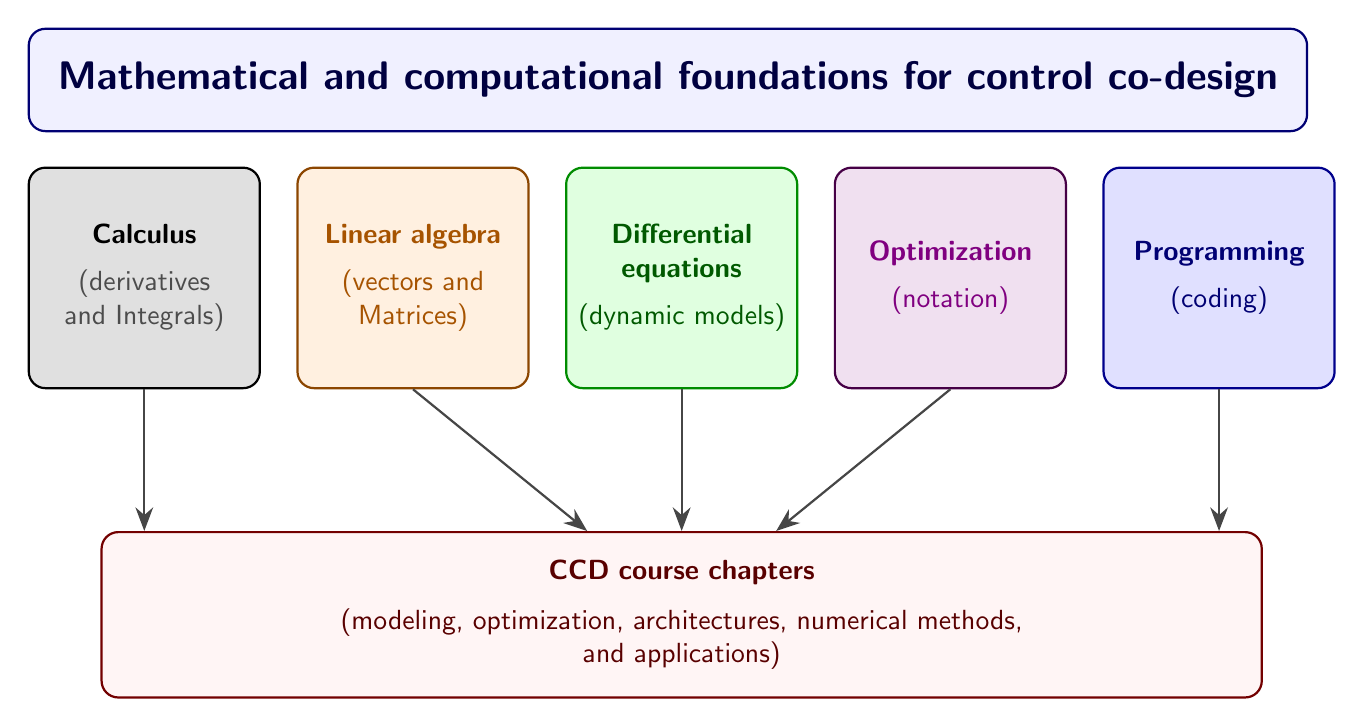
\begin{tikzpicture}[
    font=\sffamily,
    titlebox/.style={
        rectangle, rounded corners=6pt, draw=blue!45!black, thick,
        fill=blue!6, text=blue!25!black, font=\sffamily\bfseries\Large,
        minimum height=1.3cm, text width=16cm, align=center
    },
    topbox/.style={
        rectangle, rounded corners=6pt, draw=#1!55!black, thick,
        fill=#1!12, minimum height=2.8cm, minimum width=2.9cm,
        text width=2.7cm, align=center
    },
    bottombox/.style={
        rectangle, rounded corners=6pt, draw=red!45!black, thick,
        fill=red!4, minimum height=2.1cm,
        text width=14.5cm, align=center
    },
    arrow/.style={-{Stealth[length=3mm]}, thick, draw=gray!55!black}
]

% Top title box
\node[titlebox] (title) {Mathematical and computational foundations for control co-design};

% Five subject boxes, evenly spaced below the title
\node[topbox=black,  below=1.1cm of title.west, anchor=north west]
    (calc)   {\textcolor{black}{\bfseries Calculus}\\[5pt]\textcolor{black!70}{(derivatives and Integrals)}};
\node[topbox=orange, right=0.45cm of calc]
    (linalg) {\textcolor{orange!65!black}{\bfseries Linear algebra}\\[5pt]\textcolor{orange!65!black}{(vectors and Matrices)}};
\node[topbox=green,  right=0.45cm of linalg]
    (diffeq) {\textcolor{green!35!black}{\bfseries Differential\\ equations}\\[5pt]\textcolor{green!35!black}{(dynamic models)}};
\node[topbox=violet, right=0.45cm of diffeq]
    (opt)    {\textcolor{violet}{\bfseries Optimization}\\[5pt]\textcolor{violet}{(notation)}};
\node[topbox=blue,   right=0.45cm of opt]
    (prog)   {\textcolor{blue!45!black}{\bfseries Programming}\\[5pt]\textcolor{blue!45!black}{(coding)}};

% Bottom box, centered under the five boxes
\node[bottombox, below=1.8cm of diffeq.south]
    (bottom) {\textcolor{red!35!black}{\bfseries CCD course chapters}\\[6pt]
    \textcolor{red!35!black}{(modeling, optimization, architectures, numerical methods,\\ and applications)}};

% Converging arrows from each top box into the bottom box
\draw[arrow] (calc.south)   -- (bottom.north -| calc)     ;
\draw[arrow] (linalg.south) -- ($(bottom.north)+(-1.2,0)$);
\draw[arrow] (diffeq.south) -- (bottom.north)             ;
\draw[arrow] (opt.south)    -- ($(bottom.north)+(1.2,0)$) ;
\draw[arrow] (prog.south)   -- (bottom.north -| prog)     ;

\end{tikzpicture}
\end{document}
